\RequirePackage[]{silence}
%%% Warning Filter (1) {{{
\WarningFilter{latexfont}{Font shape}
\WarningFilter{latexfont}{Some font shapes were not available}
%%% }}}
\documentclass[lualatex, ja=standard, a4paper]{bxjsarticle}

\usepackage[]{../math_note}
\usepackage{booktabs}
\usepackage{xcolor}
\usepackage{graphicx}
\usepackage{here}
\usepackage{tikz}
\usetikzlibrary{cd, positioning, arrows}
\usepackage[luatex, pdfencoding=auto, colorlinks=true, allcolors=black]{hyperref}
\usepackage[backend=biber, style=alphabetic]{biblatex}
\addbibresource{reference.bib}

%% environment: question/problem {{{
\usepackage{chngcntr}
\makeatletter
    \newcounter{c@question}
    \counterwithin{c@question}{section}
    \newenvironment{question}[0]%
    {\stepcounter{c@question}\begin{itembox}[l]{問\arabic{section}.\arabic{c@question}}}%
    {\end{itembox}}%
    \newenvironment{question*}[0]%
    {\stepcounter{c@question}\begin{itembox}[l]{問}}% 
    {\end{itembox}}%
\makeatother

\makeatletter
    \newcounter{c@problem}
    \counterwithin*{c@problem}{section}
    \newenvironment{problem}[0]%
    {\stepcounter{c@problem}\begin{itembox}[l]{問題\arabic{section}.\arabic{c@problem}}}%
    {\end{itembox}}%
    \newenvironment{problem*}[0]%
    {\stepcounter{c@problem}\begin{itembox}[l]{問題}}% 
    {\end{itembox}}%
\makeatother
%% }}}

\newenvironment{myenum}[1][\roman*]
{\hfill \vspace{-0.8cm}\begin{enumerate}[label=(#1), labelindent=1cm]}
{\end{enumerate}}

\setenumerate{label=(\roman*),itemsep=3pt,topsep=7pt}

%% category
\newcommand{\ArtSt}{\mathbf{ArtSt}}
\newcommand{\Fib}[1]{\cat{Fib}(\cat{#1})}
\newcommand{\cFib}[1]{\cat{cFib}(\cat{#1})}
\newcommand{\sFib}[1]{\cat{sFib}(\cat{#1})}
\newcommand{\FibBP}[1]{\cat{Fib}^{\mathrm{bp}}(\cat{#1})}
\newcommand{\CFG}[1]{\cat{CFG}(\cat{#1})}

\newcommand{\Lim}{\operatorname*{lim}}
\newcommand{\Colim}{\operatorname*{colim}}
\newcommand{\colim}{\operatorname*{colim}}

\newcommand{\kiso}[1][{}]{\overset{#1}{\iso}}
\newcommand{\kequiv}[1][{}]{\overset{#1}{\simeq}}

%% derivation
\newcommand{\shDer}{\Omega}
\newcommand{\modDer}{\Omega}
\newcommand{\Der}{\mathrm{Der}}

%% functor
\newcommand{\ftor}[1]{\underline{#1}}
\newcommand{\ftorSh}{\mathit{Shff}}
\newcommand{\ftorFgt}{\mathit{Fgt}}

%% sites
\newcommand{\siteS}{\mathcal{S}}
\newcommand{\siteT}{\mathcal{T}}
\newcommand{\et}{\mathrm{et}}
\newcommand{\ET}{\mathrm{ET}}
\newcommand{\sm}{\mathrm{sm}}
\newcommand{\SM}{\mathrm{SM}}
\newcommand{\Zar}{\mathrm{Zar}}
\newcommand{\ZAR}{\mathrm{ZAR}}
\newcommand{\fppf}{\mathrm{fppf}}
\newcommand{\FPPF}{\mathrm{FPPF}}
\newcommand{\FPQC}{\mathrm{FPQC}}

%% covers
\newcommand{\covU}{\mathcal{U}}
\newcommand{\covV}{\mathcal{V}}
\newcommand{\covW}{\mathcal{W}}

%% utility
\newcommand{\mnewline}{\mbox{}\newline}
\newcommand{\tp}[2]{\texorpdfstring{#1}{#2}}
\newcommand{\parto}[2]{\mathrel{\mathop{\rightrightarrows}^{#1}_{#2}}}
\newcommand{\xto}[1]{\xrightarrow{#1}}
\newcommand{\step}[1]{\paragraph{\bf #1}}

%% {{{ fibered categories
\newcommand{\fib}[1]{\mathscr{#1}}
\newcommand{\fibA}{\fib{A}}
\newcommand{\fibB}{\fib{B}}
\newcommand{\fibC}{\fib{C}}
\newcommand{\fibD}{\fib{D}}
\newcommand{\fibE}{\fib{E}}
\newcommand{\fibF}{\fib{F}}
\newcommand{\fibG}{\fib{G}}
\newcommand{\fibH}{\fib{H}}
\newcommand{\fibI}{\fib{I}}
\newcommand{\fibJ}{\fib{J}}
\newcommand{\fibK}{\fib{K}}
\newcommand{\fibL}{\fib{L}}
\newcommand{\fibM}{\fib{M}}
\newcommand{\fibN}{\fib{N}}
\newcommand{\fibO}{\fib{O}}
\newcommand{\fibP}{\fib{P}}
\newcommand{\fibQ}{\fib{Q}}
\newcommand{\fibR}{\fib{R}}
\newcommand{\fibS}{\fib{S}}
\newcommand{\fibT}{\fib{T}}
\newcommand{\fibU}{\fib{U}}
\newcommand{\fibV}{\fib{V}}
\newcommand{\fibW}{\fib{W}}
\newcommand{\fibX}{\fib{X}}
\newcommand{\fibY}{\fib{Y}}
\newcommand{\fibZ}{\fib{Y}}
%% }}}

%% {{{ stacks 
\newcommand{\st}[1]{\mathcal{#1}}
\newcommand{\stA}{\st{A}}
\newcommand{\stB}{\st{B}}
\newcommand{\stC}{\st{C}}
\newcommand{\stD}{\st{D}}
\newcommand{\stE}{\st{E}}
\newcommand{\stF}{\st{F}}
\newcommand{\stG}{\st{G}}
\newcommand{\stH}{\st{H}}
\newcommand{\stI}{\st{I}}
\newcommand{\stJ}{\st{J}}
\newcommand{\stK}{\st{K}}
\newcommand{\stL}{\st{L}}
\newcommand{\stM}{\st{M}}
\newcommand{\stN}{\st{N}}
\newcommand{\stO}{\st{O}}
\newcommand{\stP}{\st{P}}
\newcommand{\stQ}{\st{Q}}
\newcommand{\stR}{\st{R}}
\newcommand{\stS}{\st{S}}
\newcommand{\stT}{\st{T}}
\newcommand{\stU}{\st{U}}
\newcommand{\stV}{\st{V}}
\newcommand{\stW}{\st{W}}
\newcommand{\stX}{\st{X}}
\newcommand{\stY}{\st{Y}}
\newcommand{\stZ}{\st{Z}}
%% }}}


\newcommand{\HOM}{\operatorname{HOM}}

\begin{document}
\title{第3章 \\ Fibered Categories}
\author{七条彰紀}
\maketitle
\tableofcontents
\vspace{10pt}

\section{Fibered Categories.}
\subsection{Motivation.}
    ``family"あるいは``object on/over a base space"
    (例えばschemes over a schemeやsheaves on a schemeなど)の
    抽象的な枠組がfibered categoryである.
    今後はfibered categoryが提供する枠組をsheaves on a siteの貼り合わせや
    stackの定義の為に活用する.

\subsection{Definitions.}
    $\stX, \cat{B}$ :: categoryと
    関手$\pi \colon \stX \to \cat{B}$を考える.
    \begin{itemize}
    \item 
        $\pi$をprojectionあるいはfibrationと呼ぶ.
    \item
        $\stX$をfibered categoryと呼ぶ.
    \item
        $\pi(O)=P$であるとき$O$は$P$の上にある($O$ is over $P$)という.
    \end{itemize}

    \newpage
\begin{Def}[Cartesian Arrow, Cartesian Lifting, Cartesian Functor, Base Preserving Natural Transformation, \cite{Olsson16} and \cite{Noohi12}]
\begin{myenum}
\item
    以下の性質(Triangle Liftingという)を満たす
    $\stX$の射$\phi \colon x \to y$をcartesian arrowという:
    (1)にあるような対象と射があるとき,
    (2)の様に射$z \to y$が\underline{ただ一つ存在し},可換と成る.
    %% {{{
    \begin{center}
    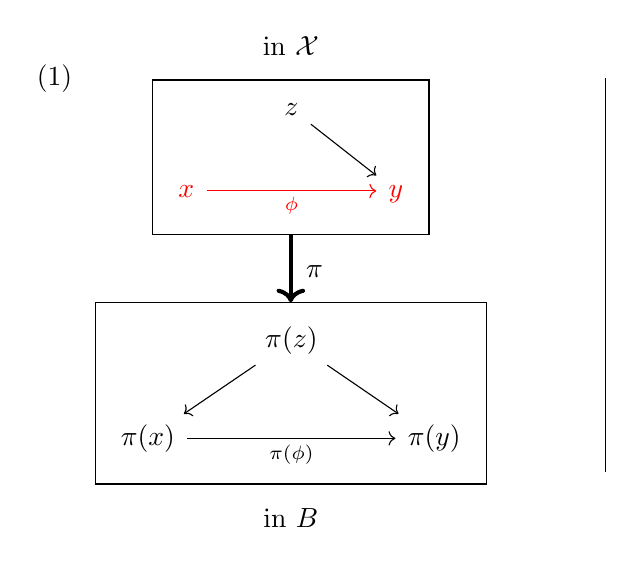
\begin{tikzpicture}[mybox/.style={draw, inner sep=5pt}]
    \node[mybox] (X) at (0,3){%
        \begin{tikzcd}
            {} & z \ar[rd]& {} \\
            \color{red}x \ar[rr, red, "\phi"'] &{}& \color{red}y
        \end{tikzcd}
    };
    \node[mybox] (B) at (0,0){%
        \begin{tikzcd}
            {} & \pi(z) \ar[rd]\ar[ld]& {} \\
            \pi(x) \ar[rr, "\pi(\phi)"'] &{}& \pi(y)
        \end{tikzcd}
    };

    \node [above=5pt of X] {in $\stX$};
    \node [below=5pt of B] {in $\cat{B}$};
    \draw [->, line width=1.5pt] (X) edge (B);
    \node at (0.3,1.55) {$\pi$};
    \draw (4,4) -- (4,-1);
    \node at (-3,4) {($1$)};
    \end{tikzpicture}
    \qquad \qquad
    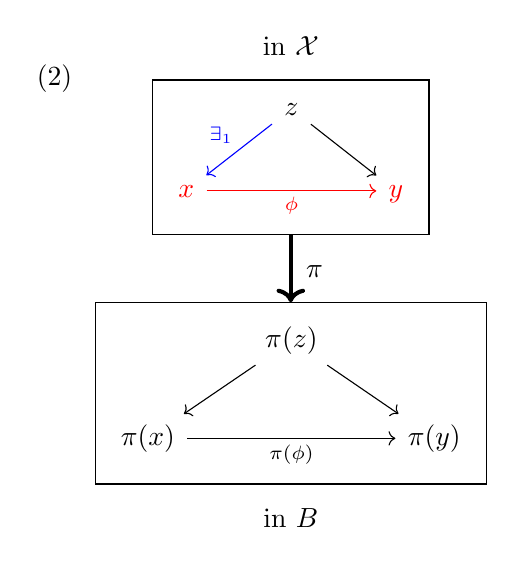
\begin{tikzpicture}[mybox/.style={draw, inner sep=5pt}]
    \node[mybox] (X) at (0,3){%
        \begin{tikzcd}
            {} & z \ar[rd] \ar[ld, blue, "\exists_1"']& {} \\
            \color{red}x \ar[rr, red, "\phi"'] &{}& \color{red}y
        \end{tikzcd}
    };
    \node[mybox] (B) at (0,0){%
        \begin{tikzcd}
            {} & \pi(z) \ar[rd]\ar[ld]& {} \\
            \pi(x) \ar[rr, "\pi(\phi)"'] &{}& \pi(y)
        \end{tikzcd}
    };

    \node [above=5pt of X] {in $\stX$};
    \node [below=5pt of B] {in $\cat{B}$};
    \draw [->, line width=1.5pt] (X) edge (B);
    \node at (0.3,1.55) {$\pi$};
    \node at (-3,4) {($2$)};
    \end{tikzpicture}
    \end{center}
    %% }}}

\item
    $y \in \stX, u \to \pi(y) \in \cat{B}$に対し,
    以下の図式を満たす
    \tablefootnote{すなわち,$\pi(x)=u, \pi(x \to y)=u \to \pi(y)$を満たす.}
    \underline{$x \in \stX$とcartesian arrow :: $x \to y \in \stX$}を,
    cartesian lifting(or cleavage) of $u \to \pi(y)$と呼ぶ.
    \begin{center}
    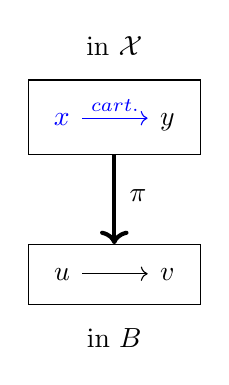
\begin{tikzpicture}[mybox/.style={draw, inner sep=5pt}]
    \node[mybox] (X) at (0,2){%
    \begin{tikzcd}
        \color{blue}x \ar[r, blue, "\text{cart.}"]& y
    \end{tikzcd}
    };
    \node[mybox] (B) at (0,0){%
    \begin{tikzcd}
        u \ar[r]& v
    \end{tikzcd}
    };

    \node [above=5pt of X] {in $\stX$};
    \node [below=5pt of B] {in $\cat{B}$};
    \draw [->, line width=1.5pt] (X) edge (B);
    \node at (0.3,1) {$\pi$};
    \end{tikzpicture}
    \end{center}

\item
    任意の$y \in \stX$と$u \to \pi(y) \in \cat{B}$に対してcartesian liftingが存在する
    $\pi \colon \stX \to \cat{B}$をfibered categoryという.
    fibered category over $\cat{B}$が成す圏を$\Fib{B}$とする.

\item
    二つのfibered category :: 
    $\pi \colon \stX \to \cat{B}, \pi' \colon \stX' \to \cat{B}$について,
    $\stX$と$\stX'$の間の射(morphism of fibered categories, cartesian functor)とは,
    functor :: $g \colon \stX \to \stX'$であって,
    $\pi, \pi'$と整合的\tablefootnote{ すなわち$\pi' \circ g=\pi$を満たす. }であり,
    cartesian arrowをcartesian arrowに写すもの.

\item
\end{myenum}
\end{Def}

\begin{Remark}
    少し圏論の言葉を整理しておく.

    対象を$0$-morphism(あるいは$0$-cell)と呼ぶ時,非負整数$k \geq 0$について,
    $k$-morphism (cell)は$(k-1)$-morphism (cell)の間の射と定義できる.
    こうして$k$-morphism (cell)は階層を成す.
    そこで,ここで定義した性質を階層別にまとめると次のように成る.
    \begin{center}
    \begin{tabular}{l|l|l}
        \hline
        arrow& arrow in a fibered category & (i) Cartesian Arrow, (ii) Cartesian Lifting \\ \hline\hline
        $0$-cell& fibered category & (iii) Existence of Cartesian Lifting \\ \hline
        $1$-cell& functor between fibered categories & (iii) Morphism of Fibered Category \\ \hline
        $2$-cell& nat. trans. between functors & (iv) Base-Preserving Natural Transformation \\
        \hline
    \end{tabular}
    \end{center}

    通常の圏同型を$1$-isoと呼び$\kiso[1]$と書く.
    この時,階層ごとのiso/equivは以下のようなものである.
    \begin{center}
        \begin{tabular}{lccl}
            iso. & $x \iso y$& $\iff$ &
                $2$つのarrow $\phi \colon x \rightleftarrows y \colon \psi$が存在し, 
                $\psi \circ \phi=\id[x], \phi \circ \psi=\id[y]$.\\ \hline\hline
            $1$-iso. & $x \kiso[1] y$& $\iff$ &
                $2$つの$1$-cell \,$\phi \colon x \rightleftarrows y \colon \psi$が存在し, 
                $\psi \circ \phi=\id[x], \phi \circ \psi=\id[y]$.\\
            $1$-equiv. & $x \kequiv[1] y$& $\iff$ &
                $2$つの$1$-cell \,$\phi \colon x \rightleftarrows y \colon \psi$が存在し, 
                $\psi \circ \phi \kiso \id[x], \phi \circ \psi \kiso \id[y]$.\\ \hline
            $2$-iso. & $x \kiso[2] y$& $\iff$ &
                $2$つの$2$-cell \,$\phi \colon x \rightleftarrows y \colon \psi$が存在し, 
                $\psi \circ \phi=\id[x], \phi \circ \psi=\id[y]$.\\
            $2$-equiv. & $x \kequiv[2] y$& $\iff$ &
                $2$つの$2$-cell \,$\phi \colon x \rightleftarrows y \colon \psi$が存在し, 
                $\psi \circ \phi \kiso[1] \id[x], \phi \circ \psi \kiso[1] \id[y]$.\\
        \end{tabular}
    \end{center}
\end{Remark}

\begin{Remark}
    $\Fib{B}$は$2$-categoryである.
    $2$-categoryは$2$-morphism ($\Fib{B}$ではnatural transformation)に
    ``vertical composition"と``horizontal composition"の二種類の合成が定まる圏である.
    詳しくはこのノートでは触れない.
\end{Remark}

\begin{Def}[Base-Preserving Natural Transformation, $\HOM$, Equivalence]
\begin{myenum}
\item
    二つのfibered category :: 
    $\pi \colon \stX \to \cat{B}, \pi' \colon \stX' \to \cat{B}$の間の$2$つの射
    $g,g' \colon \stX \to \stX'$と
    natural transformation :: $\alpha \colon g \to g'$を考える.
    \begin{center}
    \begin{tikzcd}[column sep=3cm]
        \stX \ar[rd, "\pi"]\ar[dd, shift right=3mm, "g"'{name=g}] \ar[dd, shift left=3mm, "g'"{name=gg}]& {} \\
        {} & \cat{B} \\
        \stX' \ar[ru, "\pi'"']& {}
        \ar[Rightarrow, from=g, to=gg, shorten >=2pt, shorten <=2pt, "\alpha"]
    \end{tikzcd}
    \end{center}
    任意の$x \in \stX$について,
    $\pi'(\alpha_x) \colon \pi'(g(x)) \to \pi'(g'(x))$が恒等射になるとき,
    $\alpha$をbase-preserving natural transformationという.
    
\item
    $\stX, \stX' \in \Fib{B}$について,
    $\HOM_{\cat{B}}(\stX, \stX')$を次の圏とする.
    \begin{description}
        \item[Object.] morphism of fibered category $\stX \to \stX'$.
        \item[Arrows.] base-preserving natural transformation.
    \end{description}

\item
    morphism of fibered category :: $g \colon \stX \to \stX'$が
    equivalence of fibered categoryであるとは,
    別のmorphism $h \colon \stX' \to \stX$が存在し,
    $h \circ g$と$\id[\stX]$,$g \circ h$と$\id[\stX']$の間に
    base-preserving isomorphismが存在すること
    \tablefootnote{ 基本的にはcategory of equivalenceの定義と同じである. }.
    \[ h \circ g \kiso[2] \id[\stX], g \circ h \kiso[2] \id[\stX']. \]
    二つのfibrered categoryがequivalentであるとは,
    二つの間にequivalence of fibered categoryが存在するということである.
\end{myenum}
\end{Def}

\begin{Remark}
    $2$-morphism ($2$-cell)をbase-preserving natural transformationに制限した
    fibered categoryの圏を$\FibBP{B}$とすると,
    $\HOM$は$\Hom_{\FibBP{B}}$であるし,
    equivalence of fibered categoryは$\FibBP{B}$での$2$-isoである.
\end{Remark}

\subsection{Examples.}
\begin{Example}
    morphism of schemes :: $f \colon X \to Y$を取る.
    この$f$に対し,$f$のpullbackが成す圏$\Pi(f)$を考えることが出来る.
    以下のように定義する.
    \begin{description}[labelindent=1cm]
        \item[Object.]
            pullback diagram :: 
            $\begin{tikzcd}
                P \ar[r]\ar[d]& X \ar[d, "f"]\\
                Z \ar[r]& Y
                \ar[lu, phantom, "\text{p.b.}"]
            \end{tikzcd}$
        \item[Arrow.]
            pullback diagramと整合的な射の組$(Z \to Z', P \to P')$.
    \end{description}
    $\Pi(f)$から次のようにprojectionが定まる.
    \begin{defmap}
        \pi\colon & \Pi(f)& \to& \Sch/Y \\
        {}& \begin{tikzcd}
                P \ar[r]\ar[d]& X \ar[d, "f"]\\
                Z \ar[r]& Y 
                \ar[lu, phantom, "\text{p.b.}"]
            \end{tikzcd}
        & \mapsto& [ Z \to Y ]
    \end{defmap}
    ここで注意したいのは,
    $\Pi(f)$はpullback of $f$の同型類や代表ではなく,pullback of $f$全てであることである.
    したがって$\pi \colon \Pi(f) \to \Sch/Y$は
    pullback of $f$を選択公理無しに扱う枠組を与えている.
\end{Example}

\begin{Example}
    category :: $\cat{C}$について,
    arrow category :: $\cat{C}^{\to}$を以下で定める.
    \begin{description}
        \item[Object.] $\cat{C}$の射($[x \to u]$の様に表記する).
        \item[Arrow.]
            射$[x \to u] \to [y \to v]$は
            次の図式を可換にする$x \to y, u \to v$の組: 
            $\begin{tikzcd}
                x \ar[r, dashed]\ar[d]& y \ar[d]\\
                u \ar[r, dashed]& v
            \end{tikzcd}$.
    \end{description}
    するとCartesian Liftingは$\cat{C}$がpullbackを持つことを意味し,
    Triangle Liftingはpullbackの普遍性を意味する.
\end{Example}

\begin{Example}\label{exm:representable}
    以下の関手はfibrationである.
    \begin{defmap}
        \pi\colon & \Sch/X& \to& \Sch \\
        {}& [Y \to X]& \mapsto& Y
    \end{defmap}
\end{Example}

\subsection{Propositions.}
\begin{Prop}[\cite{Vistoli07} Prop3.4]
\begin{myenum}
\item
    cartesian arrowの合成はcartesian arrowである.
\item
    $\phi \colon x \to y, \psi \colon y \to z$について,
    $\psi \circ \phi, \psi$ :: cartesian arrowならば$\psi$ :: cartesian arrow.
\end{myenum}
\end{Prop}
\begin{proof}
    Triangle Liftingのみを用いて証明できる.
    簡単なので証明は省略する.
\end{proof}

    次の命題の証明はCartesian LiftingとTriangle Liftingの使い方をよく示している.
\begin{Prop}
    $\pi \colon \stX \to \cat{B}$をfibered category over $\cat{B}$とする.
    $\stX$の射$x \to y$は以下のような二つの射の合成$x \to z \to y$に分解できる.
    \begin{itemize}
        \item $x \to z$ :: over $\id[\pi(x)]$.
        \item $z \to y$ :: cartesian, over $\pi(x \to y)$.
    \end{itemize}
\end{Prop}
%% {{{
\begin{proof}
    $\pi(\phi)$のcartesian liftingとして以下の図式(1)の$z$と$z \to y$を得る.
    さらにTriangle Liftingにより図式(2)の通り$\id[\pi(x)]$上の射$x \to z$を得る.
    \begin{center}
    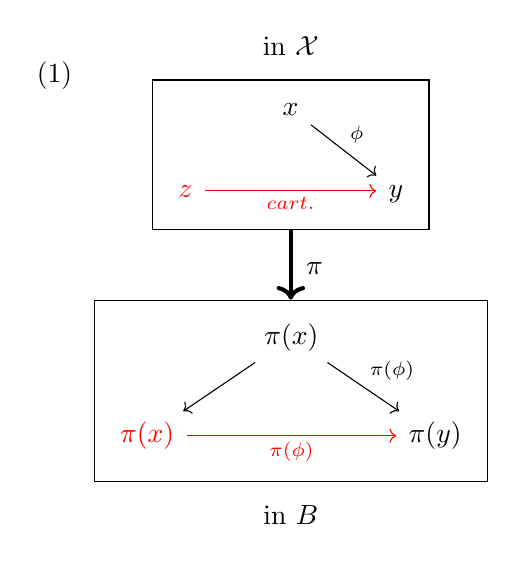
\begin{tikzpicture}[mybox/.style={draw, inner sep=5pt}]
    \node[mybox] (X) at (0,3){%
        \begin{tikzcd}
            {} & x \ar[rd, "\phi"]& {} \\
            \color{red}z \ar[rr, red, "\text{cart.}"']&{}& y
        \end{tikzcd}
    };
    \node[mybox] (B) at (0,0){%
        \begin{tikzcd}
            {} & \pi(x) \ar[rd, "\pi(\phi)"]\ar[ld, "\id"']& {} \\
            \color{red}\pi(x) \ar[rr, red, "\pi(\phi)"'] &{}& \pi(y)
        \end{tikzcd}
    };

    \node [above=5pt of X] {in $\stX$};
    \node [below=5pt of B] {in $\cat{B}$};
    \draw [->, line width=1.5pt] (X) edge (B);
    \node at (0.3,1.55) {$\pi$};
%    \draw (4,4) -- (4,-1);
    \node at (-3,4) {($1$)};
    \end{tikzpicture}
    \qquad \qquad
    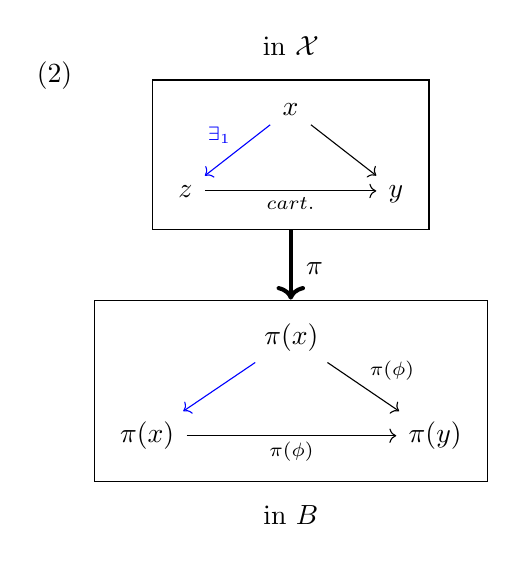
\begin{tikzpicture}[mybox/.style={draw, inner sep=5pt}]
    \node[mybox] (X) at (0,3){%
        \begin{tikzcd}
            {} & x \ar[rd] \ar[ld, blue, "\exists_1"']& {} \\
            z \ar[rr, "\text{cart.}"'] &{}& y
        \end{tikzcd}
    };
    \node[mybox] (B) at (0,0){%
        \begin{tikzcd}
            {} & \pi(x) \ar[rd, "\pi(\phi)"]\ar[ld, blue, "\id"']& {} \\
            \pi(x) \ar[rr, "\pi(\phi)"'] &{}& \pi(y)
        \end{tikzcd}
    };

    \node [above=5pt of X] {in $\stX$};
    \node [below=5pt of B] {in $\cat{B}$};
    \draw [->, line width=1.5pt] (X) edge (B);
    \node at (0.3,1.55) {$\pi$};
    \node at (-3,4) {($2$)};
    \end{tikzpicture}
    \end{center}
\end{proof}
%%}}}

\begin{Prop}\label{prop:iso_over_iso}
    $\pi \colon \stX \to \cat{B}$をfibered categoryとする.
    $\stX$の任意のcartesian morphism :: $\phi \colon x \to y$について,
    $\phi$ :: isoと$\Phi:=\pi(\phi)$ :: isoは同値.
\end{Prop}
%% {{{
\begin{proof}
    以下の図式(1)にTriangle Liftingを用いれば,
    $\phi \circ \psi=\id[y]$なる射$\psi \colon y \to x$を得る.
    さらに図式(2)に於いて,
    $\phi \circ \id[x]=\phi=\phi \circ \psi \circ \phi$とTriangle Liftingの一意性から
    $\psi \circ \phi=\id[x]$を得る.
    \begin{center}
    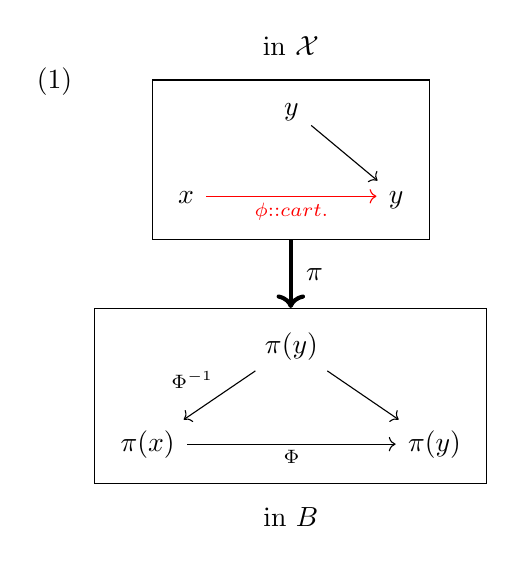
\begin{tikzpicture}[mybox/.style={draw, inner sep=5pt}]
    \node[mybox] (X) at (0,3){%
        \begin{tikzcd}
            {} & y \ar[rd, "\id"]& {} \\
            x \ar[rr, red, "\phi\text{ :: cart.}"']&{}& y
        \end{tikzcd}
    };
    \node[mybox] (B) at (0,0){%
        \begin{tikzcd}
            {} & \pi(y) \ar[rd, "\id"]\ar[ld, "\Phi^{-1}"']& {} \\
            \pi(x) \ar[rr, "\Phi"'] &{}& \pi(y)
        \end{tikzcd}
    };

    \node [above=5pt of X] {in $\stX$};
    \node [below=5pt of B] {in $\cat{B}$};
    \draw [->, line width=1.5pt] (X) edge (B);
    \node at (0.3,1.55) {$\pi$};
%    \draw (4,4) -- (4,-1);
    \node at (-3,4) {($1$)};
    \end{tikzpicture}
    \qquad \qquad
    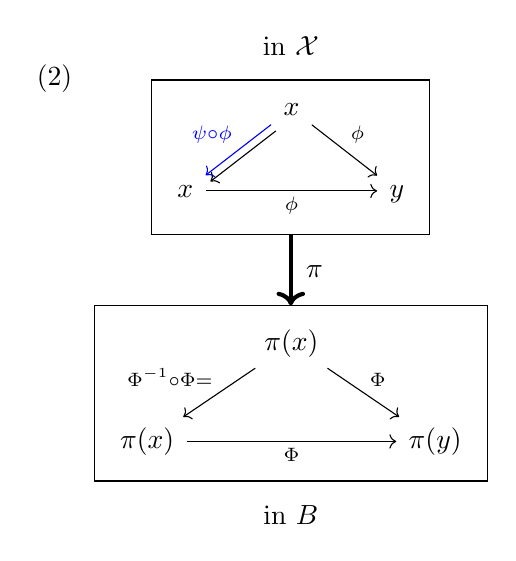
\begin{tikzpicture}[mybox/.style={draw, inner sep=5pt}]
    \node[mybox] (X) at (0,3){%
        \begin{tikzcd}
            {} & x \ar[ld, blue, "\psi \circ \phi"'] \ar[ld, shift left=1mm, "\id"] \ar[rd, "\phi"]& {} \\
            x \ar[rr, "\phi"'] &{}& y
        \end{tikzcd}
    };
    \node[mybox] (B) at (0,0){%
        \begin{tikzcd}
            {} & \pi(x) \ar[ld, "\Phi^{-1} \circ \Phi=\id"']\ar[rd, "\Phi"]& {} \\
            \pi(x) \ar[rr, "\Phi"'] &{}& \pi(y)
        \end{tikzcd}
    };

    \node [above=5pt of X] {in $\stX$};
    \node [below=5pt of B] {in $\cat{B}$};
    \draw [->, line width=1.5pt] (X) edge (B);
    \node at (0.3,1.55) {$\pi$};
    \node at (-3,4) {($2$)};
    \end{tikzpicture}
    \end{center}
\end{proof}
%% }}}

\section{Cleavage}
    Cartesian liftingは普遍性(Triangle Lifting)で特徴づけられている.
    なので同型を除いて一意であるが,厳密な意味で一意であるというものではない.
    どのCartesian liftingを用いるか選んだものがCleavage(分裂,劈開).
    これはFibered category :: $\stX$のCartesian arrowのclassを成す.
    Cleavageとfibration (resp. Fibered category)を併せたものを
    Cloven fibration (resp. Cloven fibered category)と呼ぶ.
    選択公理によって,我々は常にFibrationをCloven fibrationにできる.

\subsection{ Split Fibration }
    CleavageはCartesian arrowのclassであると書いたが,
    このclassが圏を成すと綺麗である.
    そのようなCleavageを選べるFibrationをSplit fibrationと呼ぶ.

    \begin{Def}[\cite{Olsson16}]
        $\pi \colon \stX \to \cat{B}$ :: fibered categoryとする.
        splitting of $\pi$とは,以下を満たすsubcategory :: $\cat{S} \subset \stX$のことである.
        \begin{enumerate}
            \item
                $\cat{S}$は$\stX$の任意の対象を持つ.
            \item
                $\cat{S}$の任意の射はcartesian.
            \item
                任意の$\cat{B}$の射$f \colon U \to V$と$V$上の対象$v \in \stX$について,
                $f$上の射$u \to v$がただ一つ存在する.
                (すなわち,cartesian liftingが一意に存在する.)
        \end{enumerate}
        この時,組$(\stX, \cat{S})$をsplit fibered categoryと呼ぶ.
    \end{Def}

    任意のFibrationはSplit fibrationとは限らないが,Split fibrationと圏同値である.

    \begin{Thm}
        $\pi \colon \stX \to \cat{B}$ :: fibered categoryとする.
        この時,split fibered category over $\cat{B}$ :: $(\tilde{\stX}, \cat{S})$が存在し,
        圏同値$\tilde{\stX} \kequiv \stX$が成立する.
    \end{Thm}

    \begin{proof}
        ここでは
        圏と部分圏$(\tilde{\stX}, \cat{S})$及び
        関手$\Phi \colon \tilde{\stX} \to \stX$を構成するにとどめる.
        (TODO: 
        これらがそれぞれsplit fibered category over $\cat{B}$とequivalenceであることは
        ここでは確認しない.)

        以下のように$\tilde{\stX}$を構成する.
        \begin{description}[labelindent=1cm]
            \item[Objects.]
                object :: $U \in \cat{B}$と
                morphism of fibered category :: $u \colon \cat{B}/U \to \stX$の組$(U, u)$.

            \item[Arrows.]
                射$(V, v) \to (U, u)$は
                $\cat{B}$の射$g \colon V \to U$と
                base-preserving isomorphism :: $\alpha \colon v \to u \circ g$の組$(g, \alpha)$.
                \begin{center}
                \begin{tikzcd}
                    \cat{B}/V \ar[r, "g"] \ar[rr, bend right=40mm, "v"'{name=v}]
                    & \cat{B}/U \ar[Rightarrow, from=v, "\alpha"]\ar[r, "u"]
                    & \stX
                \end{tikzcd}
                \end{center}
        \end{description}

        まずprojection functorが以下のように定まる.
        \begin{defmap}
            \tilde{\pi} \colon & \tilde{\stX}& \to& \cat{B} \\
            {}& (U, u)& \mapsto& U
        \end{defmap}
        この関手によってfibered categoryの構造が入る.

        さらに次の関手によってequivalenceが与えられる.
        \begin{defmap}
            \Phi\colon & \tilde{\stX}& \to& \stX \\
            {}& (U, u)& \mapsto& u(\id[U])
        \end{defmap}
        これがequivalenceであることは$2$-Yoneda Lemmaによる.

        最後に,splitting of $\tilde{\pi}$ :: $\cat{S}$が次で定められる.
        \begin{description}[labelindent=1cm]
            \item[Objects.]
                $\tilde{\stX}$と同じ.

            \item[Arrows.]
                $\tilde{\stX}$の射で,$(g, \id)$と表されるもの.
                すなわち,
                射$(V, v) \to (U, u)$は$\cat{B}$の射$g \colon V \to U$であって
                $v=u \circ g$であるもの.
                \begin{center}
                \begin{tikzcd}
                    \cat{B}/V \ar[r, "g"] \ar[rr, bend right=40mm, "v"'{name=v}]
                    & \cat{B}/U \ar[equal, from=v]\ar[r, "u"]
                    & \stX
                \end{tikzcd}
                \end{center}
        \end{description}
    \end{proof}

    \begin{Def}
        圏$\cat{B}$に対し,
        \begin{itemize}
            \item Cloven fibration over $\cat{B}$の圏を$\cFib{B}$,
            \item Split fibration over $\cat{B}$の圏を$\sFib{B}$
        \end{itemize}
        と書く.
        ぞれぞれ忘却関手$\sFib{B} \to \cFib{B}, \cFib{B} \to \Fib{B}$をもつ.
    \end{Def}

\section{Fiber of Fibered Categories}
\subsection{Motivation}

\subsection{Definition}
\begin{Def}[Fiber]
    $\pi \colon \stX \to \cat{B}$をfibered categoryとする.
    任意の$b \in \cat{B}$について,
    以下で定める圏を$\stX_b$あるいは$\stX(b)$と書き,
    fiber of $\pi$ at (over) $b$と呼ぶ:
    \begin{description}[labelindent=1cm]
        \item[Object.] $\pi(x)=b$となるobject :: $x \in \stX$.
        \item[Arrow.] $\pi(\phi)=\id[b]$となるarrow :: $\phi \in \stX$.
    \end{description}

    morphism of fibered category :: $g \colon \stX \to \stY$から
    fiberの間に誘導される射を$g_B \colon \stX_B \to \stY_B$と書く.
\end{Def}
\begin{Remark}
    標語的には次のように定義されている.
    \[
        \stX_b=\stX(b):=``
        \pi^{-1} \left(
        \begin{tikzcd}
            b \ar[loop right, "\id"]
        \end{tikzcd}
        \right)"
    \]
    
    また,
    morphism of schemes :: $f \colon X \to B$のfiberが
    $f^{-1}(b)$と表現されることと比較せよ。
\end{Remark}

$\stX$は上で定義したfiberとcartesian liftingによって
contravariant functorに成ることが予想される.
しかしこれは一般には正しくない.
正確には,fibered categoryのfiberは一般にpsuedo-functorとなる.
このことは後に証明する.
\begin{Def}[Psuedo-functor (weak 2-functor)] \label{def:psuedofunctor}
    (以下のURLを参照せよ: \url{https://stacks.math.columbia.edu/tag/003G}.)
    $2$-圏$\cat{C}$から$2$-圏$\cat{D}$への
    psuedo-functor :: $F \colon \cat{C} \to \cat{D}$とは,
    $\cat{C}$のobjectを$\cat{D}$のobjectへ,
    $\cat{C}$のarrowを$\cat{D}$のarrowへ対応させるものであり,
    以下を満たす.
    
    \begin{enumerate}[label=(\alph*)]
        \item
            任意の$c \in \cat{C}$について
            $2$-isomorphism $\alpha_{c} \colon F(\id[c]) \to \id[F(c)]$が存在する.
        \item 任意の$f \colon c \to d, g \colon d \to e \in \cat{C}$について
            $2$-isomorphism $\alpha_{g, f} \colon F(g \circ f) \to F(g) \circ F(f)$が存在する.
        \item
            $f \colon x \to y, g \colon y \to z, h \colon z \to w$について
            以下の等式が成り立つ.
            \begin{center}
            \begin{tikzcd}[column sep=huge]
                F(x) \ar[r, bend left, "F(f)", ""{name=Fful}] \ar[r, bend right, "F(f)"', ""{name=Ffdl}]&
                F(y) \ar[r, bend left, "\id", ""{name=id}] \ar[r, bend right, "F(\id)"', ""{name=Fid}]&
                F(y)
                
                \arrow[Rightarrow, from=Fful, to=Ffdl, "\mathrm{id}_{F(f)}", shorten <=2pt]
                \arrow[Rightarrow, from=id,   to=Fid,  "\alpha_{y}", shorten <=2pt]
            \end{tikzcd}
            =
            \begin{tikzcd}[column sep=huge]
                F(x) \ar[r, bend left, "F(f)", ""{name=Ffur}]\ar[r, bend right, "F(f)"', ""{name=Ffdr}]& F(y)
                \arrow[Rightarrow, from=Ffur, to=Ffdr, "\alpha_{\mathrm{id}_y, f}", shorten <=2pt]
            \end{tikzcd}
            \end{center}
            
            \begin{center}
            \begin{tikzcd}
                F(x) \ar[r] \ar[r, bend left] \ar[rrr, bend left=40pt]& F(y) \ar[r] \ar[rr, bend left]& F(z) \ar[r]& F(w)
            \end{tikzcd}
            \end{center}
    \end{enumerate}
\end{Def}

\subsection{Propositions}
\begin{Lemma} \label{lem:cart_ump}
    $\pi \colon \stX \to \cat{B}$をfibered categoryとする.
    任意の$\cat{B}$の射$f \colon b \to b'$と$x \in \stX(b')$について,
    $f$と$x$に対するcartesian liftingは,
    同型を除いて一意に存在する.
\end{Lemma}
\begin{proof}
    存在はfibered categoryの定義から明らか.
    一意性はcartesian liftingが普遍性を持つことを
    Triangle Liftingを用いて示せば良い.
\end{proof}

\begin{Lemma}
    $\pi \colon \stX \to \cat{B}$をfibered categoryとする.
    このとき,fiber of $\pi$はpsuedo-functorである.
\end{Lemma}
\begin{proof}
    $b \in \cat{B}$について,$\stX(b)$は既に既に定義した.
    $\cat{B}$の射$\phi \colon b' \to b$について,
    関手$\stX(\phi) \colon \stX(b) \to \stX(b')$は次のように定められる.
    まず$u \in \stX(b)$について,
    $\stX(\phi)(u)$は
    $\phi$による$u$のpullback :: $\phi^* u$ (cartesian lifting of $\phi$)である.
    次に$\stX(b)$の射$\lambda \colon u \to v$
    ($\stX(b)$の定義から$\pi(\lambda)=\id$を満たす)について,
    下の図式にtriangle liftingを用いて$\phi^*u \to \phi^*v$を得る.
    %% {{{
    \begin{center}
    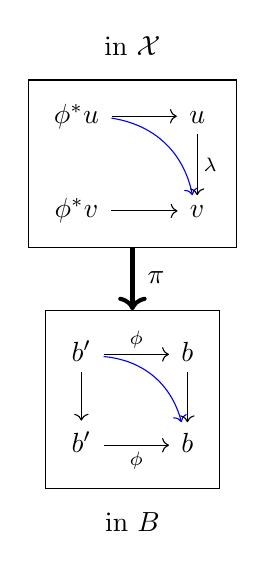
\begin{tikzpicture}[mybox/.style={draw, inner sep=5pt}]
    \node[mybox] (X) at (0,3){%
        \begin{tikzcd}
            \phi^*u \ar[r]\ar[rd, blue, bend left=35pt]& u \ar[d, "\lambda"]\\
            \phi^*v \ar[r] & v
        \end{tikzcd}
    };
    \node[mybox] (B) at (0,0){%
        \begin{tikzcd}
            b' \ar[r, "\phi"] \ar[d, "\id"']\ar[rd, blue, bend left=35pt]& b \ar[d, "\id"]\\
            b' \ar[r, "\phi"'] & b
        \end{tikzcd}
    };

    \node [above=5pt of X] {in $\stX$};
    \node [below=5pt of B] {in $\cat{B}$};
    \draw [->, line width=1.5pt] (X) edge (B);
    \node at (0.3,1.55) {$\pi$};
    \end{tikzpicture}
    \end{center}
    %% }}}

    定義(\ref{def:psuedofunctor})にある条件(a)については,
    各$b \in \cat{B}$について,
    命題(\ref{prop:iso_over_iso})を用いれば同型の存在が分かる.
    条件(b)については,
    各$f \colon c \to d, g \colon d \to e \in \cat{C}$と各$b \in \cat{B}$について
    補題(\ref{lem:cart_ump})を用いれば
    $\stX(g \circ f)(b) \iso \stX(f) \circ \cat{B}(g)(b)$が得られる.
    あとはこの同型が自然である(すなわち自然変換を定める)ことを確かめれば良い.
\end{proof}
この事実は次のセミナーで用いる.

\begin{Thm}[$2$-Yoneda Lemma (Fibered Yoneda Lemma)]
    $\pi \colon \stX \to \cat{B}$ :: fibered categoryとする.
    以下のように関手を定める.
    \begin{defmap}
        Y\colon & \cat{B}& \to& \Fib{B}\\
        {}& U& \mapsto& \cat{B}/U
    \end{defmap}
    ここで$\cat{B}/U$は例(\ref{exm:representable})にあるとおり
    fibered category over $\cat{B}$である.

    この時,圏同値$\HOM_{\cat{U}}(Y(U), \stX) \to \stX(U)$が成り立つ.
\end{Thm}
\begin{proof}
    (TODO)
\end{proof}

\begin{Remark}
    この定理から,$\stX(U)$を「空間」$\stX$の$U$-rational pointsと考えることが出来る.
    また,この定理から関手$Y$が
    $U \in \cat{B}$のfibered category over $\cat{B}$への「昇格」を与えていることが分かる.
\end{Remark}

\begin{Cor}
    圏同値$U, V \in \cat{B}$について$Y(U) \simeq Y(V)$と$U \iso V$は同値.
\end{Cor}

\section{Grothendieck Construction} \label{sec:gro_const}
    今,fibered categoryからfiberとしてpsuedo-functorを構成した.
    実はこの逆が出来る.
    \begin{Def}[Grothendieck Construction, \cite{Olsson16}, \cite{Noohi12}]
        psuedo-functor :: $P \colon \cat{B} \to \Cat/\cat{B}$について,
        以下のように圏$\int P$を定義する.
        \begin{description}[labelindent=1cm]
            \item[Object.] $b \in \cat{B}$と$x \in P(b)$の組$(b, x)$.
            \item[Arrow.] $\phi \colon b \to b'$と$\Phi \colon P(\phi)(x) \to x'$の組$(\phi, \Phi)$.
        \end{description}
        射の合成は$(\psi, \Psi) \circ (\phi, \Phi)=(\psi \circ \phi, \Phi \circ P(\psi)(\Phi))$で与えられる.
        
        この圏によって以下の関手が定まる.
        \begin{defmap}
            \int \colon & \left\{ \parbox{2.3cm}{psuedo-functor \\ \quad \ $\cat{B} \to \Cat$} \right\}&
                \to& \sFib{B} \\
            {}& P& \mapsto& \int P
        \end{defmap}
    \end{Def}

    \begin{Example}
        scheme :: $S$について,
        representable functor :: $\ftor{S}$は$\Sch/S$に対応する.
    \end{Example}

    \begin{Example}
        presheaf of set :: $F \colon \cat{C} \to \Set$は
        $\bigsqcup_{c \in \cat{C}} F(c)$に対応する.
    \end{Example}

    \begin{Remark}
        David I. Spivak ``Category theory for scientists"によると,
        Grothendieck Constructionを最初に構成したのはGrothendieckではない.
        例えばMacLaneが以前から扱っている.
    \end{Remark}

    \begin{Def}[weak/strict $2$-equivalence]
        関手$F \colon \cat{C} \rightarrow \cat{D}$が
        weak $2$-equivalenceであるとは,以下が成り立つこと:
        逆向きの関手$\cat{C} \leftarrow \cat{D} \colon G$と
        二つの自然変換$\alpha \colon GF \to \id[\cat{C}], \beta \colon FG \to \id[\cat{D}]$が存在し,
        \begin{itemize}
            \item 各$c \in \cat{C}, d \in \cat{D}$について$\alpha_{c}, \beta_{d}$は同型であり,
            \item 射$\phi \in \Arr(\cat{C}), \psi \in \Arr(\cat{D})$について$\alpha_{\phi}, \beta_{\psi}$も同型.
        \end{itemize}
        $\alpha_{\phi}, \beta_{\psi}$が恒等射であるときはstrict $2$-equivalenceという.
    \end{Def}

    \begin{Thm}[Grothendieck Construction give Category Equivalence]
        Grothendieck Construction
        \[
            \int \colon
            \left\{ \parbox{2.3cm}{psuedo-functor \\ \quad \ $\cat{B} \to \Cat$} \right\} \to \cFib{B}
        \]
        はstrict $2$-equivalenceである.
        また,このあとに忘却関手$\cFib{B} \to \Fib{B}$を続けると,
        weak $2$-equivalenceとなる.
    \end{Thm}
    \begin{proof}
        \cite{Vistoli07} \S 3.1.3に詳しい証明がある.
        あるいは,
        P. T. Johnstone
            ``Sketches of an Elephant: A Topos Theory Compendium vol.1 (Oxford Logic Guides 43)"
        に証明がある.
    \end{proof}
    
    \begin{Remark}
        $\Fib{B}$と``anafunctor"の圏がstrict $2$-equivalenceである,
        という述べ方もあるようだが,
        ``anafunctor"を用いる理由が特に無いので,このノートでは導入しない.
    \end{Remark}

    \begin{Remark}
        この定理から,
        psuedo-functorの理論とfibered categoryの理論は殆ど同じ,と言える.
        また,今後現れるstackなどはpsuedo-functorに対して定義され,
        一見,fibered categoryの理論は扱う必要性がなくなる.
        
        しかし実際には,fibered categoryの方がpsuedo-functorより構成しやすい,
        あるいは全体の性質を理解しやすいという面がある.
        また技術的な有利としては,
        fibered categoryはcleavage(例えばpullback, fiber product等)を選択する必要がなく,
        例えば,pullbackの貼り合わせ(貼り合わせの際には同型での変形が必要に成る)を自然に扱うことが出来る
        \footnote
        {
            もう少し具体的な例としては,
            trivial familyの貼り合わせで出来るlocally trivial familyも扱える.
            詳しい例は私のDeformation Theoryに関するノートを読んで欲しい.
        }.
        
        また,直観としては,fibered categoryはfamilyである.
        ここから得られるfiberは正にfiber of familyである.
        そのためfibered categoryは大域的,psuedo-functorは局所的だと考えられる.

        (TODO: あとで分かったらもっと追記する.)
    \end{Remark}

\section{Category Fibered in Groupoids/Sets}
\subsection{Motivation}
    Category Fibered in Groupoidsは「綺麗すぎる」fibered categoryであるが,
    我々が研究する範囲では珍しいものではない.
    

\subsection{Definition}
    \begin{Def}[Groupoid]
        任意の射が同型射である圏をgroupoidと呼ぶ.
    \end{Def}

    \begin{Remark}
        群は対象がただ一つで任意の射が同型であるものとみなせるため,
        groupoidにはこの名前がある.

        群以外の極めて単純なgroupoidとして,
        集合を射が恒等射しかない圏(離散圏)とみなしたものがある.
        そのため,逆に恒等射しか無い圏もsetと呼ぶ.
    \end{Remark}

    \begin{Def}[Category fibered in groupoids/sets]
        $\pi \colon \stX \to \cat{B}$をfibered categoryとする.
        任意の$b \in \cat{B}$について,
        $\pi$の$b$におけるfiber$\stX(b)$がgroupoid (set)であるとき,
        $\stX$をcategory fibered in groupoids (sets)と呼ぶ.
    \end{Def}
    category fibered in groupoidsは次のように定義しても同値である.

    \begin{Def}[Category fibered in groupoid (Another Definition)]
        任意の射がcartesianであるfibered categoryをcategory fibered in groupoidsと呼ぶ.
        すなわち,
        以下の$2$条件が成立する圏$\stX$と関手$\pi \colon \stX \to \cat{B}$を
        category fibered in groupoidsと呼ぶ.
        \begin{enumerate}[label=(\roman*)]
        \item
            以下の図式(1)において,
            上の箱と下の箱が$\pi$で対応し,下の箱にある図式が可換であるとする.
            この時,図式(2)のように上の箱にある図式を可換にし,
            $\pi$での対応を保つ射$z \to x$がただ一つ存在する.
            %% {{{
            \begin{center}
            \begin{tikzpicture}[mybox/.style={draw, inner sep=5pt}]
            \node[mybox] (X) at (0,3){%
                \begin{tikzcd}
                    {} & z \ar[rd]& {} \\
                    x \ar[rr] &{}& y
                \end{tikzcd}
            };
            \node[mybox] (B) at (0,0){%
                \begin{tikzcd}
                    {} & \pi(z) \ar[rd]\ar[ld]& {} \\
                    \pi(x) \ar[rr] &{}& \pi(y)
                \end{tikzcd}
            };

            \node [above=5pt of X] {in $\stX$};
            \node [below=5pt of B] {in $\cat{B}$};
            \draw [->, line width=1.5pt] (X) edge (B);
            \node at (0.3,1.55) {$\pi$};
            \draw (3.7,4) -- (3.7,-1);
            \node at (-3,4) {($1$)};
            \end{tikzpicture}
            \qquad
            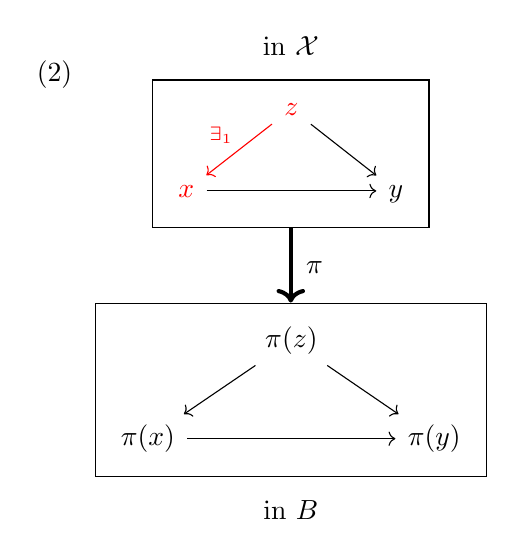
\begin{tikzpicture}[mybox/.style={draw, inner sep=5pt}]
            \node[mybox] (X) at (0,3){%
                \begin{tikzcd}
                    {} & \color{red}z \ar[rd] \ar[ld, red, "\exists_1"']& {} \\
                    \color{red}x \ar[rr] &{}& y
                \end{tikzcd}
            };
            \node[mybox] (B) at (0,0){%
                \begin{tikzcd}
                    {} & \pi(z) \ar[rd]\ar[ld]& {} \\
                    \pi(x) \ar[rr] &{}& \pi(y)
                \end{tikzcd}
            };

            \node [above=5pt of X] {in $\stX$};
            \node [below=5pt of B] {in $\cat{B}$};
            \draw [->, line width=1.5pt] (X) edge (B);
            \node at (0.3,1.55) {$\pi$};
            \node at (-3,4) {($2$)};
            \end{tikzpicture}
            \end{center}
            %% }}}

        \item
            $y \in \stX, u \to \pi(y) \in \cat{B}$に対し,
            以下の図式を満たす
            \tablefootnote{すなわち,$\pi(x)=u, \pi(x \to y)=u \to \pi(y)$を満たす.}
            \underline{$x \in \stX$と射$x \to y \in \stX$}が存在する.
            \begin{center}
            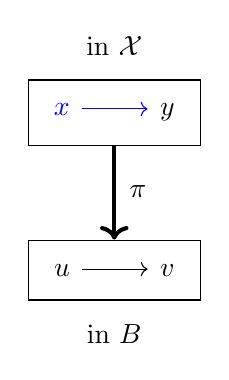
\begin{tikzpicture}[mybox/.style={draw, inner sep=5pt}]
            \node[mybox] (X) at (0,2){%
            \begin{tikzcd}
                \color{blue}x \ar[r, blue]& y
            \end{tikzcd}
            };
            \node[mybox] (B) at (0,0){%
            \begin{tikzcd}
                u \ar[r]& v
            \end{tikzcd}
            };

            \node [above=5pt of X] {in $\stX$};
            \node [below=5pt of B] {in $\cat{B}$};
            \draw [->, line width=1.5pt] (X) edge (B);
            \node at (0.3,1) {$\pi$};
            \end{tikzpicture}
            \end{center}
        \end{enumerate}
    \end{Def}
    \begin{proof}
        \cite{SP} 003V\footnote{ \url{https://stacks.math.columbia.edu/tag/003V} }.
    \end{proof}

\section{Equivalence of Fibered Categories}
    Fibered categoryの一般論の最後に,
    この直後に扱うことと成るEquivalenceを扱う.
    
    この節では
    fibered categories :: $\pi \colon \stX \to \cat{B}, \pi' \colon \stX' \to \cat{B}$と,
    これらの間の射$g \colon \stX \to \stX'$を考える.

\subsection{Definition}
    \begin{Def}[Equivalence]
        $g$がequivalence of fibered categoriesであるとは,
        別の射$h \colon \stX' \to \stX$が存在し,
        $g \circ h, h \circ g$が
        それぞれ恒等関手とbase-preserving isomorphicであるということである.

        この時,$\stX \simeq \stX'$と書き,
        $h$はpsuedo-inverse of $g$と呼ばれる.
    \end{Def}
    \begin{Remark}
        比較すれば分かるとおり,
        equivalence of fibered categoriesは,
        通常の圏同値の定義に``base-preserving"という条件が追加されただけである.
    \end{Remark}

\subsection{Propositions}
    \begin{Prop}
        fiberedとは限らない圏$\cat{C}, \cat{D}$と
        その間の関手$F \colon \cat{C} \to \cat{D}$について,
        $F$が圏同値であることは以下の$2$条件が同時に成立することと同値.
        \begin{description}
            \item[Fully Faithfulness.] \mbox{}\\
                任意の$c,c' \in \cat{C}$について,\mbox{}\\
                関手$F$が与えるclassの対応$\Hom_{\cat{C}}(c, c') \to \Hom_{\cat{D}}(F(c), F(c'))$は全単射である.

            \item[Essential Surjectivity.] \mbox{}\\
                任意の$d \in \cat{D}$について,$F(c) \iso d$となる対象$c \in \cat{C}$が存在する.
        \end{description}
    \end{Prop}
    \begin{proof}
        \cite{Awodey10} Prop7.26を参照せよ.
    \end{proof}

    \begin{Prop}[\cite{Olsson16} Prop3.1.18, 3.1.10]
        $b \in \cat{B}$について,
        $g$を$\stX(b)$に制限して得られる関手を$g_b \colon \stX(b) \to \stX'(b)$とする.
        \begin{enumerate}[label=(\alph*)]
        \item $g$ :: fully faithful
                $\iff$ 任意の$b \in \cat{B}$について,$g_{b}$ :: fully faithful.
        \item $g$ :: equivalence
                $\iff$ 任意の$b \in \cat{B}$について,$g_{b}$ :: equivalence
                    \tablefootnote{こちらは通常の圏同値}.
    \end{enumerate}
    \end{Prop}
    \begin{proof}
        いずれも$\implies$は自明なので$\impliedby$を示す.

        (i)の証明の概略は以下の通り.
        まず$\Hom_{\cat{C}}(c, c'), \Hom_{\cat{D}}(F(c), F(c'))$を
        \begin{align*}
            \Hom_{\cat{C}}(c, c')
            =&\bigsqcup_{h \in \Hom_{\cat{B}}(\pi(c), \pi(c'))}
            \left\{\parbox{2.85cm}{morphisms $c \to c'$, \\ \qquad\ \ over $h$}\right\}, \\
            \Hom_{\cat{D}}(F(c), F(c'))
            =&\bigsqcup_{h \in \Hom_{\cat{B}}(\pi(c), \pi(c'))}
            \left\{\parbox{4cm}{morphisms $F(c) \to F(c')$, \\ \qquad\qquad\ over $h$}\right\}
        \end{align*}
        と分解する.
        そして各$h$についてsession 4の命題4.2
        (射はcartesian arrowと$\id$に写る射の合成に分解できる)を用いる.
        すると各成分について全単射を構成できる.

        (TODO: proof of (ii))
    \end{proof}

\printbibliography[title=参考文献]
\end{document}
